
Time series from 227 existing Roll decay tests conducted at SSPA Maritime Dynamics Laboratory have been collected. The tests were conducted with scale models with length in the range of 3 to 6 meters. The tests were originally conducted in commercial projects for new buildings of merchant ships. The main parameters of the ships are summarized in non dimensional form in figure \ref{fig:ship_parameters}. 

\begin{figure}[H]
    \centering
    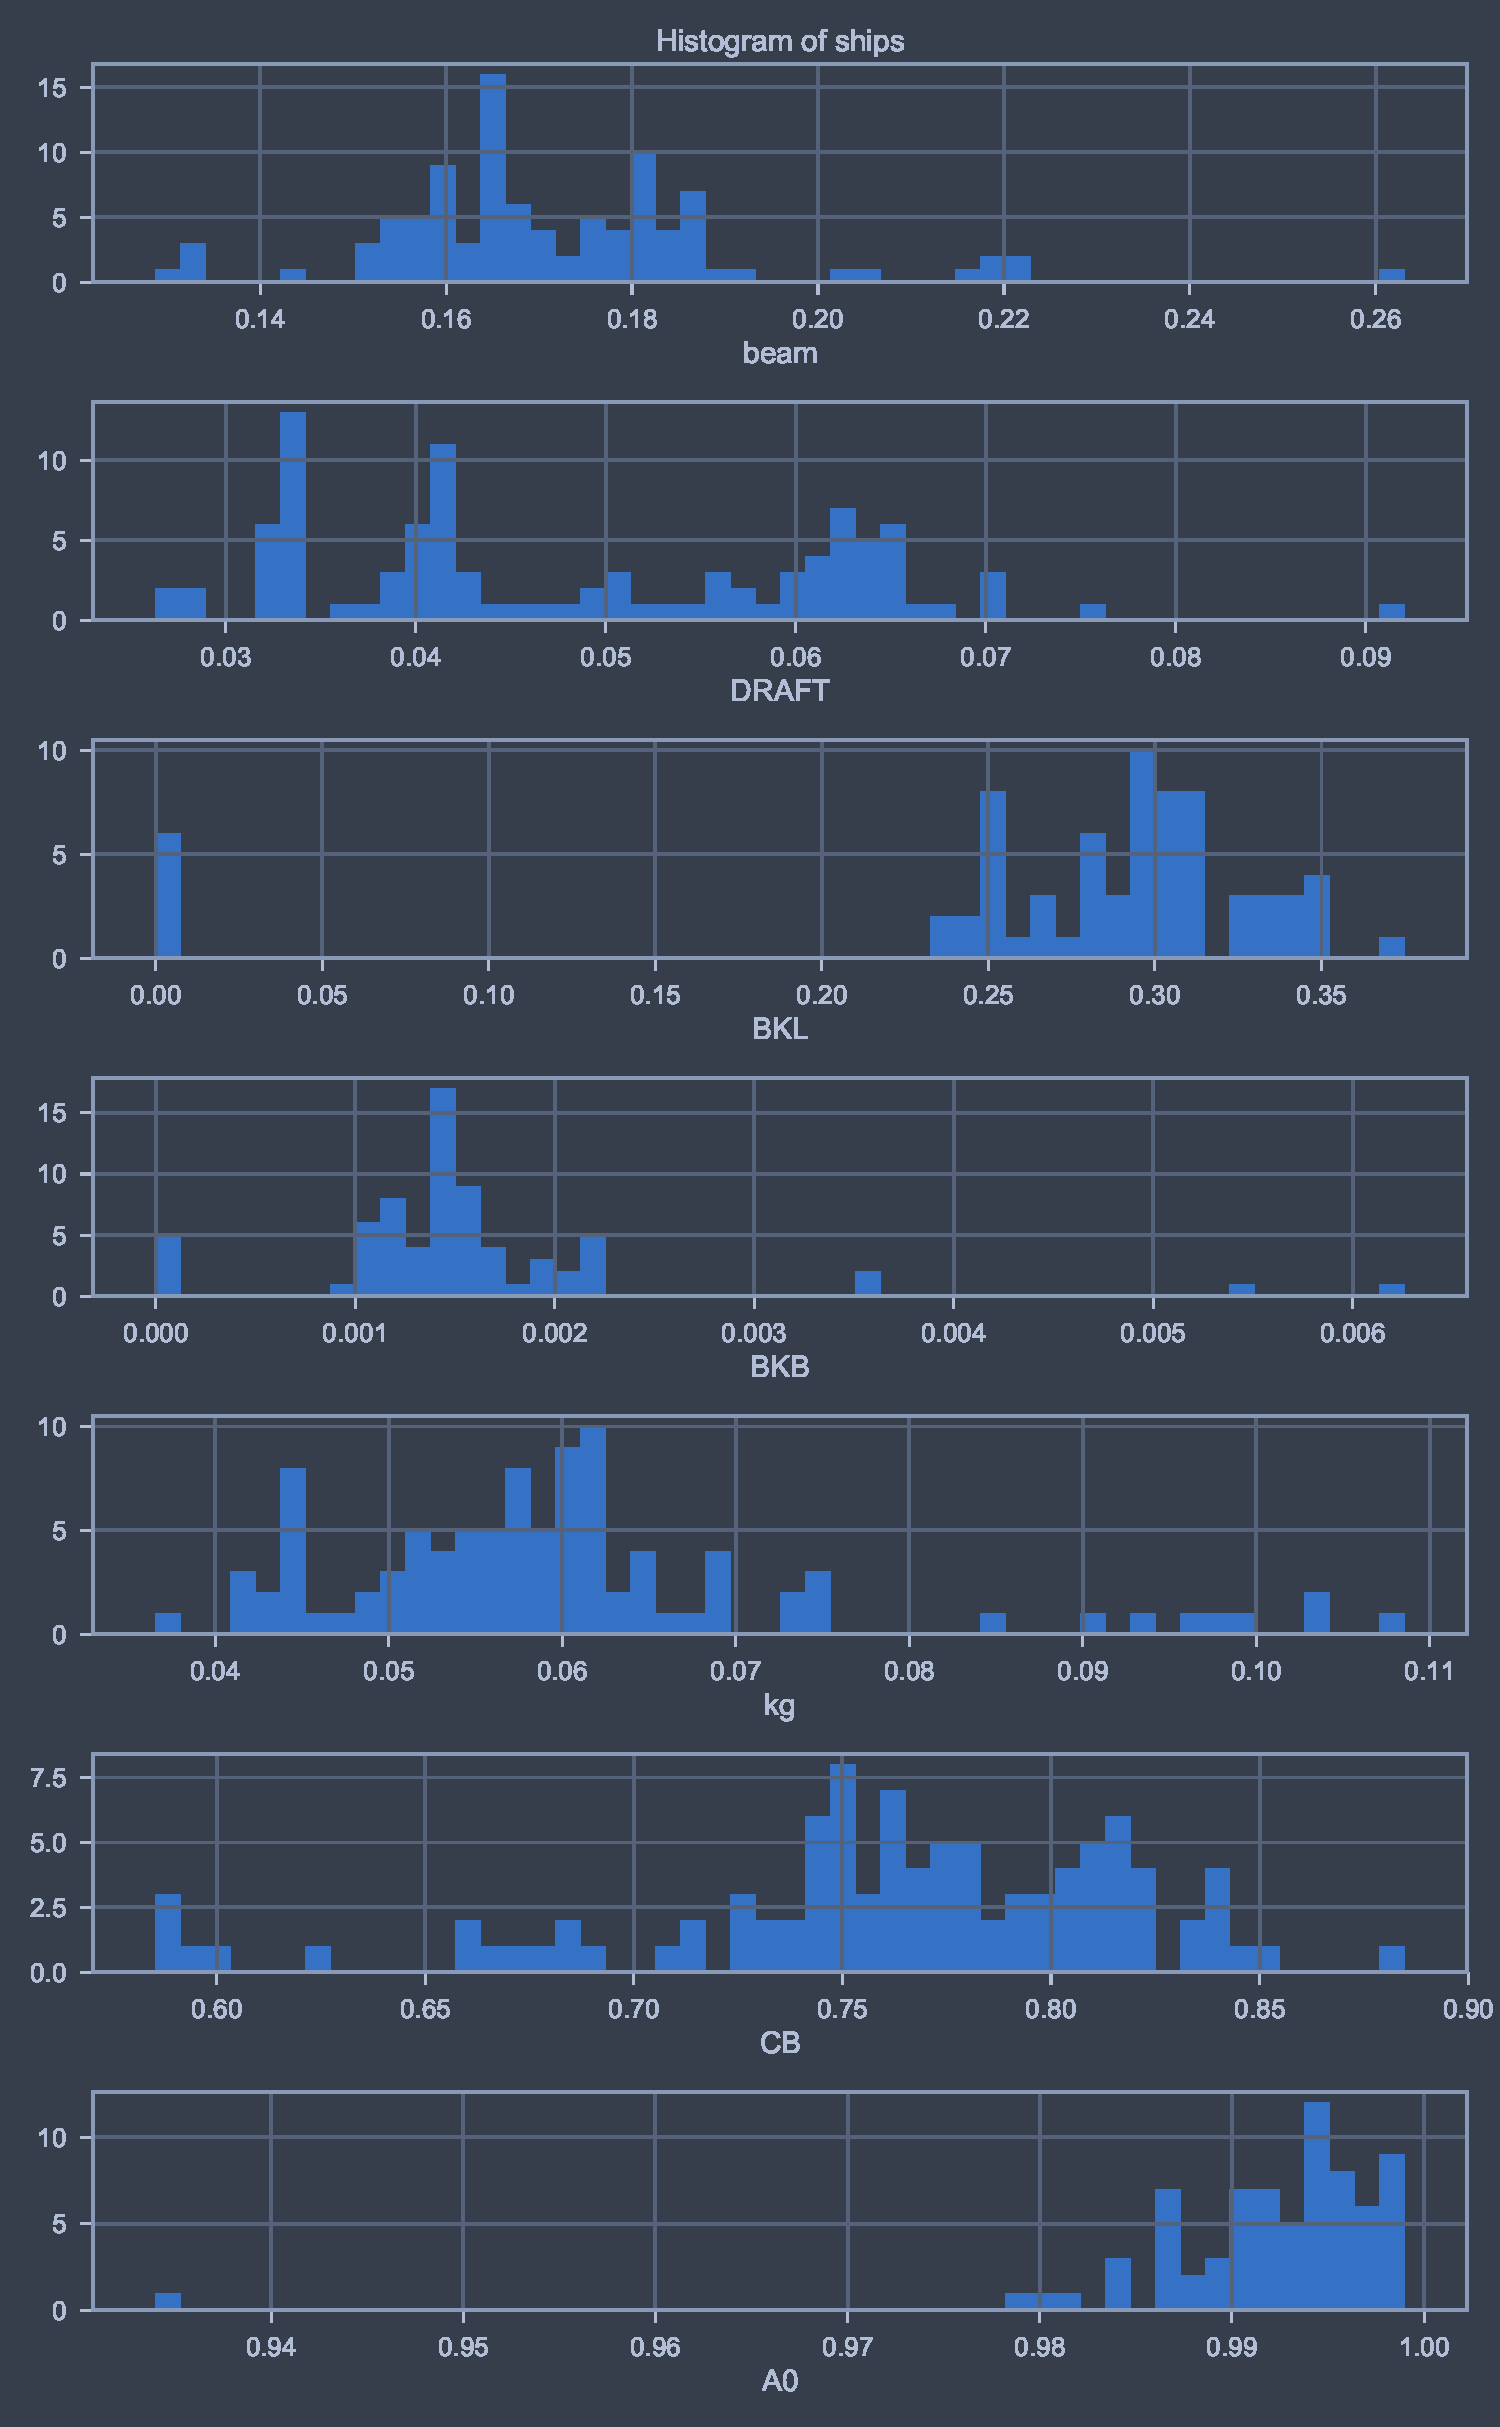
\includegraphics[width=0.8\columnwidth]{figures/ship_parameters.pdf}
    \caption{Histograms of ship parameters from the model tests, all parameters except CB and A0 have been normalized with Lpp}
    \label{fig:ship_parameters}
\end{figure}

The roll decay test database is used to build a roll damping database. The parameter identification technique as described in section \ref{se:PIT} was used to extract damping coefficients from the roll decay tests. Whether the linear model (equation \ref{eq:roll_decay_equation_himeno_linear}), quadratic model (equation \ref{eq:roll_decay_equation_himeno_quadratic}) or cubic model (equation \ref{eq:roll_decay_equation_cubic}) should be used to build the roll damping database was investigated. Simulations with identified models were conducted and the accuracy of the fit was evaluated with the $R^2$ score coefficient, based on model test and simulation time series.
The average $R^2$ was 0.995 for the cubic model, 0.993 for the quadratic and 0.986 for the linear model. Since the quadratic model has almost the same accuracy as the cubic model it was selected to be used for the roll damping database.
